% CoRA-centered working draft, 2026-09-21.
% Evidence and editorial decisions: PAPER_CORA_NOTES_20260921.md.
% Existing test.tex and all experiment artifacts are preserved.
% Compile from the repository root. References are embedded below.
\documentclass[10pt,twocolumn]{article}
\newif\ifconferencestyle
\IfFileExists{spconf.sty}{\usepackage{spconf}\conferencestyletrue}{%
  \usepackage[a4paper,left=20mm,right=20mm,top=20mm,textheight=229mm]{geometry}\conferencestylefalse}
\usepackage{amsmath,amssymb,graphicx,booktabs,pgfplots,hyperref}
\pgfplotsset{compat=1.18}
\newcommand{\U}{\mathbf{U}}
\newcommand{\X}{\mathbf{X}}
\newcommand{\HH}{\mathbf{H}}
\newcommand{\C}{\mathcal{C}}
\newcommand{\cora}{CoRA}

\title{CoRA: Randomized Decoding for Quantized Update Inversion\\
and Its Reconstruction Limits Across Bit Widths}
\ifconferencestyle
  \name{Anonymous Author(s)}
  \address{Anonymous Affiliation}
\else
  \author{Anonymous Author(s)\\Anonymous Affiliation}
  \date{}
\fi

\begin{document}
\maketitle

\begin{abstract}
Quantizing a model update leaves multiple numerical updates compatible with
the transmitted observation. We study \cora{} (Consistency-Ranked restart
Attack), which explores this ambiguity through randomized decoding,
source separation, and feature inversion. The sender quantizes
deterministically; randomness enters only when the attacker samples
admissible values within the observed quantization cells. A public score
combining feature agreement and total variation ranks the resulting
reconstructions, and selected candidates receive further optimization.
We evaluate this procedure on VGG16/ImageNet local updates using signed
per-tensor quantization from 8 to 4 bits. As precision decreases, the
selected reconstruction's LPIPS increases from 0.5558 to 0.8085 and PSNR
decreases from 12.0568 to 11.5028 dB. Reconstructions at 8 bits retain
visible structure in some examples, whereas the 4-bit outputs exhibit
substantial loss of object and scene detail. Relative to naive
dequantization, the benefit of randomized decoding varies with bit width
and metric. These results characterize both the behavior and the limits
of \cora{} under the evaluated reconstruction budget.
\end{abstract}

\noindent\textbf{Index Terms---}Update inversion, randomized decoding,
quantization, source separation, reconstruction quality.

\section{Introduction}
\label{sec:intro}
Model updates can reveal information about the data used to compute them.
Deep Leakage from Gradients reconstructs training inputs through gradient
matching~\cite{zhu2019deep}. The Cocktail Party Attack (CPA) instead uses
independent component analysis to separate the inputs mixed in fully
connected gradients and updates~\cite{kariyappa2023cocktail}.
In a compressed communication setting, however, an attacker receives a
quantized representation rather than the original numerical update.
The reconstruction procedure must therefore choose how to decode it.

Naive dequantization assigns every received code its cell center. This is
a natural deterministic estimate, but it represents only one numerical
completion of the observation. A randomized decoder can generate other
admissible completions and pass them through the same reconstruction
pipeline. The important empirical questions are whether candidate search
helps recover image structure and how the resulting quality changes when
the quantization cells become wider.

We address these questions with \cora{}, a randomized decoding and
candidate-selection procedure. It samples values inside the observed
cells, separates source features from each sampled update, and inverts
those features into images. A score computable from the public model and
the recovered features determines which candidates receive additional
optimization. The output is one selected reconstruction; source or image
averaging is not part of the evaluated method.

The paper makes three contributions. First, it specifies a
compression-compatible randomized decoder and its integration with a
CPA-based source-separation and feature-inversion pipeline. Second, it
defines a public candidate-ranking procedure and reports its actual
computational budget. Third, it characterizes reconstruction quality
across an 8/7/6/5/4-bit per-tensor sweep, using paired naive-decoding
controls, image metrics, and qualitative reconstructions. Our emphasis
is the observed dependence on bit width, including settings where
randomized search provides little or no improvement.

\section{Observation Model}
\label{sec:observation}
\subsection{Client update and attacker knowledge}
We consider an exposed single-client local update in a federated learning
round. The client starts from public weights and performs full-batch SGD.
The convolutional feature extractor is frozen, while the fully connected
layers are trained. The attacker knows the starting model, batch size,
and local training configuration, and observes the quantized fully
connected updates with their decoding metadata. The attack uses the
first fully connected weight matrix. Training images, labels, true
features, and uncompressed updates are unavailable to the attack and its
candidate selector.

Let $\HH=[\phi(x_1),\ldots,\phi(x_B)]^\top$ contain the frozen features
entering the first fully connected layer. If the gradient at local step
$t$ is $\mathbf{A}_t\HH$, with loss averaging included in
$\mathbf{A}_t$, then the local update is
\begin{equation}
 \U=\mathbf{W}^{(T)}-\mathbf{W}^{(0)}
     =-\eta\left(\sum_{t=0}^{T-1}\mathbf{A}_t\right)\HH.
 \label{eq:mixture}
\end{equation}
This expresses the multi-step update as a mixture of fixed input
features and motivates CPA-based source separation. The sign convention
matches the stored after-training-minus-initial update. Our observation
model does not assume access to an individual update concealed by secure
aggregation.

\subsection{Signed per-tensor quantization}
For each tensor, the deterministic quantizer uses
\begin{equation}
 \begin{aligned}
 Q_b&=2^{b-1}-1,\qquad s=\frac{\|\U\|_\infty}{Q_b},\\
 q_j&=\operatorname{round}_{\mathrm{even}}(U_j/s).
 \end{aligned}
 \label{eq:quantizer}
\end{equation}
Codes lie in $[-Q_b,Q_b]$, giving $2^b-1$ numerical levels, and one
FP32 scale $s$ is stored per tensor. A zero tensor is represented by zero
codes and unit scale. Arithmetic and scale storage follow the FP32
implementation. Throughout this paper, bit width refers to numerical
code precision. The experiment artifacts store codes in int8 with
additional scale and packet metadata; this sweep is not a measurement of
packed communication size.

For positive $s$, the ideal interior cell for code $q_j$ extends from
$s(q_j-\tfrac12)$ to $s(q_j+\tfrac12)$. Ties-to-even rounding,
finite precision, and the requirement to reproduce the tensor scale
determine the actual admissible endpoints. We write $\C(q,s)$ for the
set of FP32 tensors that reproduce the received codes and scale.
Naive decoding uses $U^{\mathrm{ctr}}_j=sq_j$.

\section{CoRA: Randomized Decoding and Candidate Ranking}
\label{sec:cora}
\subsection{Sampling compatible numerical updates}
\cora{} generates candidate first-FC matrices
$\widetilde\U^{(m)}\in\C(q,s)$. For non-anchor coordinates, it
draws uniformly between the admissible cell endpoints and casts to FP32.
An extremal coordinate is anchored to a scale-compatible maximum.
The implementation checks that the resulting matrix reproduces both the
codes and the stored scale under re-encoding. This is a bounded sampling
rule, without a learned or calibrated prior over the original update.

Naive decoding and one randomized draw are different procedures. The
former always returns the cell center; the latter chooses another
compatible value. In the ideal interior-cell model, center decoding has
coordinate error at most $s/2$, whereas a sampled completion can differ
from the true value by almost $s$. Randomization therefore does not
guarantee a more accurate numerical update. Its purpose here is to
explore alternative inputs to the nonlinear reconstruction pipeline.

\subsection{Source separation and feature inversion}
Each decoded first-FC matrix is processed using FastICA initialization
followed by gradient refinement of the source separation. Source rows
are aligned to the center-decoded reference using Hungarian assignment
on absolute cosine similarity. Alignment changes permutation and sign
only; it neither rescales source norms nor averages sources across
members. The absolute recovered sources are used as feature-inversion
targets, denoted $z_{m,i}=|\hat h_{m,i}|$.

For each candidate, feature inversion optimizes images $\hat\X_m$ to
match these targets through the public feature extractor. The
implemented backend is a modified CPA-based pipeline: FastICA and
gradient refinement produce the features, and feature inversion produces
the images. The reported results should be interpreted for this backend.

\subsection{Public screening and continuation}
\label{sec:screen}
After an initial feature-inversion budget, \cora{} computes
\begin{equation}
 J_m=\frac{1}{B}\sum_{i=1}^{B}
 \left[1-\cos\!\left(\phi(\hat x_{m,i}),z_{m,i}\right)\right]
 +0.1\,\mathrm{TV}_{\mathrm{norm}}(\hat\X_m).
 \label{eq:score}
\end{equation}
The score is evaluated on a pixel-boxed clone in normalized model-input
space. It uses only the public model, decoded sources, and current
candidate images. Here, consistency refers to feature agreement,
regularized by total variation; this score does not replay local training
or compare a recompressed image-induced update with the packet.

In the evaluated configuration, $K=8$ sampled candidates each receive
5,000 feature-inversion iterations. The three lowest-scoring candidates
continue to a total of 25,000 iterations, preserving optimizer and
scheduler states. The scheduler horizon is 25,000 from the first step,
and ties use ascending member index. The candidate ranked first at
screening remains the primary reported output after continuation. We do
not choose among the finalists using private image metrics or average
their reconstructions.

This yields the following sequence for a fixed observed packet:
\begin{enumerate}
 \item Decode the center reference and generate $K$ compatible samples.
 \item Separate source features for each decoding and align the sources.
 \item Run initial feature inversion and rank candidates by $J_m$.
 \item Continue the retained candidates and return the originally
       rank-1 candidate at the final optimization budget.
\end{enumerate}
The naive control uses center decoding and the same reconstruction
backend, with 25,000 feature-inversion iterations.

\section{Experimental Evaluation}
\label{sec:experiments}
\subsection{Settings and evaluation protocol}
We evaluate pretrained VGG16 on a fixed ImageNet batch, holding the
victim data and local-training configuration constant across bit widths.
The client uses $B=16$, $T=10$, and SGD learning rate $10^{-3}$, with
zero momentum, zero weight decay, and disabled dropout. Only fully
connected parameters are trained. The quantizer uses one scalar scale
per parameter tensor in every condition.

FastICA uses an iteration cap of 200 and tolerance $10^{-6}$, followed
by 4,000 refinement iterations at learning rate $10^{-3}$. The source
count is $B$. Randomized decoding uses seeds $1234+1000003m$ for
$m=0,\ldots,7$. Feature inversion uses Adam with initial learning rate
0.1 and a cosine scheduler; its feature and total-variation weights are
1 and 0.1. These settings are held fixed across the bit sweep.

We report mean PSNR, SSIM, and VGG-based LPIPS~\cite{zhang2018lpips}.
Higher PSNR and SSIM, and lower LPIPS, indicate better image agreement.
Private evaluation begins only after the public candidate selection has
been fixed. Because source separation is permutation-ambiguous, the
evaluator performs one pixel-MSE Hungarian assignment per candidate and
reuses it for all three metrics and the displayed reconstructions.
LPIPS uses FP32 RGB images mapped from $[0,1]$ to $[-1,1]$.
All reconstructed images contribute to the reported means.

\subsection{ImageNet: reconstruction across bit widths}
\label{sec:bits}
\begin{table}[t]
\centering
\caption{VGG16/ImageNet local-update reconstruction under deterministic
signed per-tensor quantization. Naive denotes cell-center decoding;
\cora{} denotes the public rank-1 candidate from $K=8$ samples.
Every reported endpoint has 25,000 feature-inversion iterations.
The candidate-search budgets differ, as detailed in Section~\ref{sec:budget}.}
\label{tab:bits}
\small
\setlength{\tabcolsep}{4pt}
\begin{tabular}{clrrr}
\toprule
Bits & Method & PSNR $\uparrow$ & SSIM $\uparrow$ & LPIPS $\downarrow$\\
\midrule
8 & Naive & 12.0569 & 0.2924 & 0.5594\\
8 & \cora{} & 12.0568 & 0.3070 & 0.5558\\
\addlinespace
7 & Naive & 11.7955 & 0.2764 & 0.6118\\
7 & \cora{} & 11.8314 & 0.2827 & 0.6332\\
\addlinespace
6 & Naive & 11.6397 & 0.2596 & 0.6961\\
6 & \cora{} & 11.6675 & 0.2690 & 0.6659\\
\addlinespace
5 & Naive & 11.5524 & 0.2620 & 0.7826\\
5 & \cora{} & 11.5458 & 0.2558 & 0.7490\\
\addlinespace
4 & Naive & 11.5197 & 0.2921 & 0.8071\\
4 & \cora{} & 11.5028 & 0.2576 & 0.8085\\
\bottomrule
\end{tabular}
\end{table}

\begin{figure}[t]
\centering
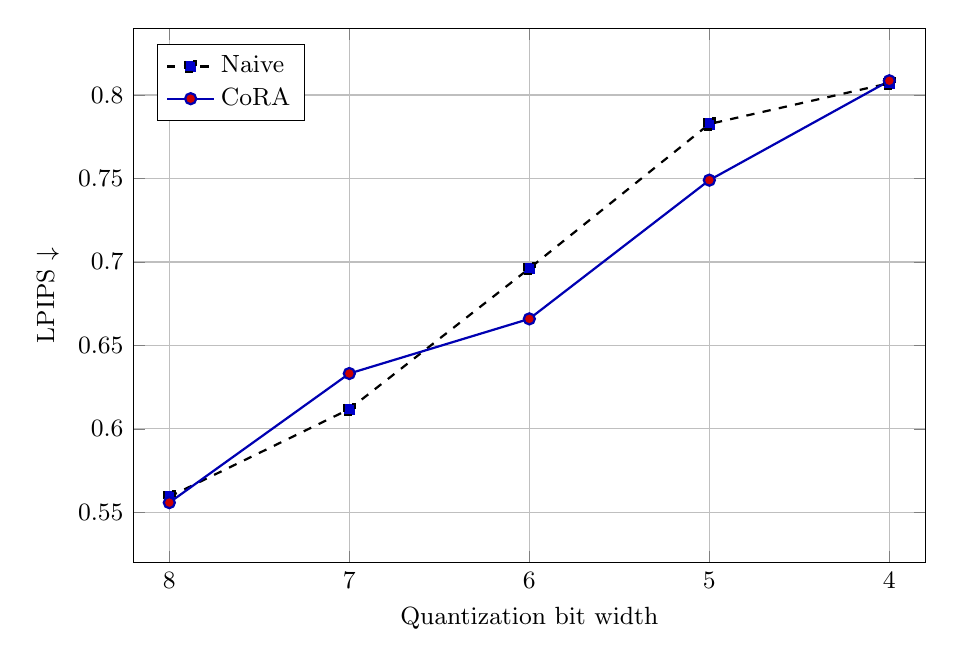
\begin{tikzpicture}
\begin{axis}[
 width=0.96\columnwidth,height=0.69\columnwidth,
 xlabel={Quantization bit width},ylabel={LPIPS $\downarrow$},
 xmin=3.8,xmax=8.2,xtick={4,5,6,7,8},x dir=reverse,
 ymin=0.52,ymax=0.84,grid=major,
 tick label style={font=\small},label style={font=\small},
 legend style={font=\small,at={(0.03,0.97)},anchor=north west},
 legend cell align=left]
\addplot+[color=black,dashed,mark=square*,thick] coordinates {
 (8,0.5594061017) (7,0.6118270941) (6,0.6961209550)
 (5,0.7826303653) (4,0.8070732467)};
\addlegendentry{Naive}
\addplot+[color=blue!70!black,mark=*,thick] coordinates {
 (8,0.5558413193) (7,0.6331724599) (6,0.6659042519)
 (5,0.7489930727) (4,0.8085191771)};
\addlegendentry{\cora{}}
\end{axis}
\end{tikzpicture}
\caption{Perceptual reconstruction quality as precision decreases from
8 to 4 bits. Points are the fixed-batch means in Table~\ref{tab:bits};
connecting lines guide the eye.}
\label{fig:bits}
\end{figure}

Table~\ref{tab:bits} and Fig.~\ref{fig:bits} show progressive degradation
in the selected \cora{} output as precision decreases. LPIPS increases
from 0.5558 at 8 bits through 0.6332, 0.6659, and 0.7490 to 0.8085 at
4 bits. PSNR decreases from 12.0568 to 11.5028 dB. SSIM does not follow
a monotonic curve, so the three metrics should be considered together.

The comparison with naive decoding is mixed. At 8 bits, \cora{} improves
SSIM and LPIPS with nearly unchanged PSNR. At 6 bits, all three metrics
improve. At 5 bits, LPIPS improves while PSNR and SSIM decrease. At
7 bits, PSNR and SSIM improve but LPIPS worsens. At 4 bits, the selected
candidate is worse than the naive control on all three metrics. Thus
the measured benefit of candidate search depends on precision and the
quality measure; it does not remove the degradation at low bit widths.

\subsection{CIFAR-100: reconstruction across bit widths}
\label{sec:cifar100}
% Draft-only space reservation. Replace this box after evaluation.
% Add the actual CIFAR-100 model, attack backend, decoding, budget, and
% matching protocol to Section 4.1 before interpreting the results.
% The existing CIFAR-100 handoff concerns original CPA/FC2 with center
% decoding; it is not automatically a randomized CoRA comparison.
% Do not merge results from different backends into a controlled ablation.
\noindent\fbox{%
\begin{minipage}{\dimexpr\columnwidth-2\fboxsep-2\fboxrule\relax}
\small
\textbf{Reserved for CIFAR-100 experiments.}
No results are reported in this placeholder.
\par\medskip
\textbf{Experimental setup:} model, attack method, decoding,
optimization budget, and evaluation protocol.
\par\medskip
\centering
\begin{tabular}{crrr}
\toprule
Bits & PSNR $\uparrow$ & SSIM $\uparrow$ & LPIPS $\downarrow$\\
\midrule
8 & --- & --- & ---\\
7 & --- & --- & ---\\
6 & --- & --- & ---\\
5 & --- & --- & ---\\
4 & --- & --- & ---\\
\bottomrule
\end{tabular}
\par\medskip
\raggedright
\textbf{Reconstruction examples and interpretation:}
to be added after evaluation.
\par\vspace{8mm}
\end{minipage}}

\subsection{Individual draws and the selected candidate}
\label{sec:individual}
Table~\ref{tab:individual} clarifies the distinction between naive
decoding, the first random draw, and the selected \cora{} output at
4 bits. The first draw is member 00, whereas the public selector chooses
member 06. Member 00 appears here because it ranked third and was also
continued to the final budget. It is an existing candidate endpoint,
not a separately evaluated $K=1$ procedure.

\begin{table}[t]
\centering
\caption{Existing 4-bit endpoints at 25,000 feature-inversion iterations.
The first-draw row is descriptive, as explained in
Section~\ref{sec:individual}. No candidate averaging is used.}
\label{tab:individual}
\small
\setlength{\tabcolsep}{3pt}
\begin{tabular}{lrrr}
\toprule
Decoding/output & PSNR $\uparrow$ & SSIM $\uparrow$ & LPIPS $\downarrow$\\
\midrule
Naive center & 11.5197 & 0.2921 & 0.8071\\
First draw (member 00) & 11.5558 & 0.2614 & 0.8055\\
\cora{} (public rank 1) & 11.5028 & 0.2576 & 0.8085\\
\bottomrule
\end{tabular}
\end{table}

The first draw has slightly better PSNR and LPIPS than the selected
candidate. Public feature agreement is therefore not equivalent to
private image similarity in this example. We retain the publicly
selected output in Table~\ref{tab:bits} to evaluate the specified attack,
including this limitation of its selector.

\subsection{Visual structure at higher and lower precision}
\label{sec:qualitative}
The complete 8-bit and 4-bit reconstructions are shown in
Fig.~\ref{fig:qualitative}. At 8 bits, some reconstructions retain
recognizable person, animal, and background structure, although contrast
and fine detail remain weak and other examples are dominated by noise.
At 4 bits, the selected reconstructions largely consist of mottled
texture and faint shapes with substantially reduced correspondence to
the original objects and scenes. This visual contrast complements the
LPIPS trend. The intermediate bit widths quantify how quality changes
between these endpoints rather than defining a universal cutoff.

\subsection{Computational budget and scope}
\label{sec:budget}
The recorded randomized search performs
$8\times5{,}000+3\times20{,}000=100{,}000$ feature-inversion iterations
per bit width. The separate naive control adds 25,000 iterations,
bringing the recorded total to 125,000. Source separation is performed
for each of the eight samples and for the center reference. Thus final
per-candidate iteration counts match, while total search budgets do not.
The comparison measures the outputs of these procedures; it does not
establish a compute-matched advantage from randomized decoding alone.

The sweep holds one victim batch and one set of candidate seeds fixed.
It characterizes this setting, without estimating variability across
independent batches or complete search runs. Comparisons to other
datasets, quantization granularities, source-separation backends, or
image-matching protocols require separate evidence.

\section{Discussion}
\label{sec:discussion}
Lower precision widens the numerical ambiguity available to the attacker,
but the additional possible completions do not supply information about
which one matches the private update. Equation~\ref{eq:mixture} also
imposes source structure that independent cell sampling does not
explicitly enforce. Coarse completions can therefore provide poor
inputs to source separation even when they reproduce the packet.
This is a possible explanation of the observed degradation, not a
mechanism isolated by the current sweep.

Candidate ranking presents a second limitation. The feature targets in
Eq.~\ref{eq:score} are themselves estimated from the compressed update.
A reconstruction may fit those targets without resembling the private
image, as the individual-candidate comparison illustrates. In addition,
exact re-encoding of a sampled numerical update does not establish that
local training on the final reconstructed images would reproduce the
same packet. That image-induced update constraint was not evaluated in
this experiment.

The results consequently support a conditional account of reconstruction
limits: with this sampler, selector, backend, and budget, 8-bit outputs
retain structure in some examples, and lowering precision to 4 bits
substantially degrades that structure. The intermediate-bit measurements
describe the quality trajectory. They do not establish that any bit
width protects against other attack procedures or larger search budgets.

\section{Conclusion}
\cora{} reconstructs quantized local updates by sampling compatible
decodings and ranking the resulting image candidates using a public
feature-based score. Its per-tensor VGG16/ImageNet bit sweep shows
decreasing PSNR and worsening LPIPS from 8 to 4 bits, accompanied by a
substantial loss of visual structure. Randomized decoding offers mixed
improvements over naive dequantization and does not compensate for
coarse quantization in the evaluated 4-bit setting. The measured quality
curves and reconstructions describe where the current procedure retains
image information and where its limitations become pronounced.

\begin{thebibliography}{9}
\bibitem{zhu2019deep}
L. Zhu, Z. Liu, and S. Han,
``Deep leakage from gradients,''
in \emph{Advances in Neural Information Processing Systems}, vol. 32, 2019.
% https://papers.neurips.cc/paper_files/paper/2019/hash/60a6c4002cc7b29142def8871531281a-Abstract.html

\bibitem{kariyappa2023cocktail}
S. Kariyappa, C. Guo, K. Maeng, W. Xiong, G. E. Suh,
M. K. Qureshi, and H.-H. S. Lee,
``Cocktail Party Attack: Breaking aggregation-based privacy in federated
learning using independent component analysis,''
in \emph{Proc. International Conference on Machine Learning},
vol. 202, pp. 15884--15899, 2023.
% https://proceedings.mlr.press/v202/kariyappa23a.html

\bibitem{zhang2018lpips}
R. Zhang, P. Isola, A. A. Efros, E. Shechtman, and O. Wang,
``The unreasonable effectiveness of deep features as a perceptual metric,''
in \emph{Proc. IEEE Conference on Computer Vision and Pattern Recognition},
2018.
% https://openaccess.thecvf.com/content_cvpr_2018/html/Zhang_The_Unreasonable_Effectiveness_CVPR_2018_paper.html
\end{thebibliography}

\clearpage
\onecolumn
\appendix
\section{Complete Qualitative Reconstructions}
The following panels reproduce the existing evaluation contact sheets.
They include all image rows in the evaluated batch. Columns within each
panel are ground truth, naive decoding, and the three randomized
candidates ordered by their public screening ranks. The primary
\cora{} output is public rank 1, in the third column. The other finalists
are shown for context and do not replace the primary reported output.

\begin{figure}[!ht]
\centering
\includegraphics[width=0.48\textwidth,height=0.76\textheight,keepaspectratio]{quantization_aware_cpa/results_private/signed_int8_screen3_repair_B16_T10_20260918/evaluation_final_20260918/figures_with_baseline_20260918/contact_sheet_b8_25000_with_baseline.png}
\hfill
\includegraphics[width=0.48\textwidth,height=0.76\textheight,keepaspectratio]{quantization_aware_cpa/results_private/signed_int4_randomized8_screen3_fia_B16_T10_20260918_sweep/evaluation_recovery_20260918/figures_with_baseline_20260918/contact_sheet_b4_25000_with_baseline.png}
\caption{Complete final reconstructions at 8 bits (left) and 4 bits
(right), at 25,000 feature-inversion iterations. The first column in
each panel is ground truth; the second is naive dequantization; the
third is the selected \cora{} output. Public ranks 2 and 3 follow.
The same victim-image ordering is used in both panels, with offline
pixel-MSE assignment applied separately to each candidate.}
\label{fig:qualitative}
\end{figure}
\end{document}
